\documentclass[tikz,border=10pt]{standalone}
\usepackage{tikz}
\usepackage{amsmath,amssymb}
\usetikzlibrary{arrows.meta,positioning,shapes}
\definecolor{politoNavy}{RGB}{0, 43, 91}
\definecolor{examred}{RGB}{192, 41, 43}
\definecolor{deepblue}{RGB}{31, 78, 121}
\definecolor{deepdiveTeal}{RGB}{0, 128, 128}
\definecolor{intuitiongreen}{RGB}{39, 174, 96}

\begin{document}
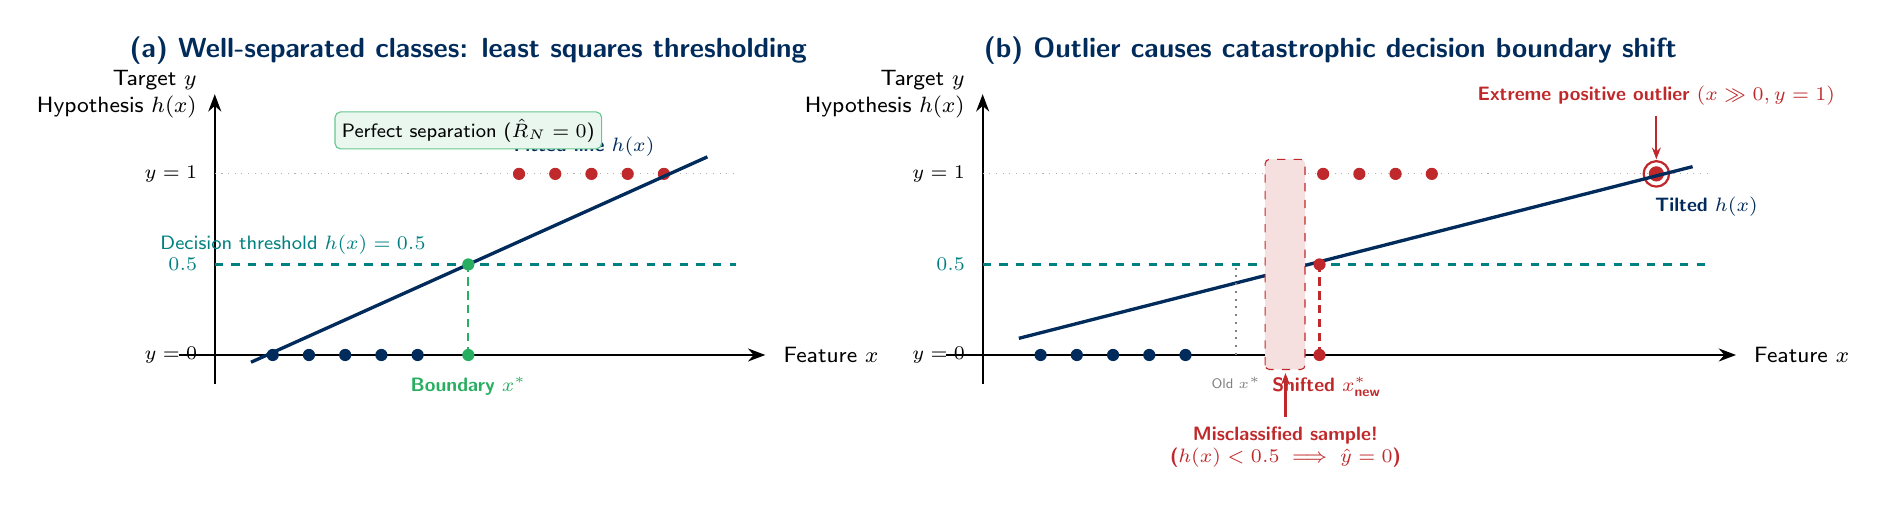
\begin{tikzpicture}[scale=0.92]
  % Left Panel: Clean Separable Dataset
  \begin{scope}[shift={(0,0)}]
    \node[font=\bfseries\sffamily, text=politoNavy] at (3.5, 4.2) {(a) Well-separated classes: least squares thresholding};
    % Axes
    \draw[-{Stealth[length=2.2mm]}, thick] (-0.5, 0) -- (7.6, 0) node[right=1mm, font=\footnotesize\sffamily] {Feature $x$};
    \draw[-{Stealth[length=2.2mm]}, thick] (0, -0.4) -- (0, 3.6) node[left=1mm, font=\footnotesize\sffamily, align=right] {Target $y$\\Hypothesis $h(x)$};
    
    % y=0 and y=1 labels
    \node[left=1mm, font=\scriptsize\sffamily] at (0, 0) {$y = 0$};
    \node[left=1mm, font=\scriptsize\sffamily] at (0, 2.5) {$y = 1$};
    \draw[dotted, gray!60] (0, 2.5) -- (7.2, 2.5);

    % Threshold line y=0.5 (height 1.25)
    \draw[dashed, thick, deepdiveTeal] (0, 1.25) -- (7.2, 1.25) node[pos=0.15, above, font=\scriptsize\sffamily, text=deepdiveTeal] {Decision threshold $h(x) = 0.5$};
    \node[left=1mm, font=\scriptsize\bfseries\sffamily, text=deepdiveTeal] at (0, 1.25) {$0.5$};

    % Class 0 points (y=0)
    \foreach \x in {0.8, 1.3, 1.8, 2.3, 2.8} {
      \fill[politoNavy] (\x, 0) circle (2.4pt);
    }
    % Class 1 points (y=1, y-coord=2.5)
    \foreach \x in {4.2, 4.7, 5.2, 5.7, 6.2} {
      \fill[examred] (\x, 2.5) circle (2.4pt);
    }

    % Linear regression line: passes through (3.5, 1.25)
    \draw[very thick, politoNavy] (0.5, -0.1) -- (6.8, 2.735) node[pos=0.92, above left=1mm, font=\scriptsize\bfseries\sffamily] {Fitted line $h(x)$};

    % Boundary vertical projection at x = 3.5
    \draw[thick, densely dashed, intuitiongreen] (3.5, 0) -- (3.5, 1.25);
    \fill[intuitiongreen] (3.5, 1.25) circle (2.4pt);
    \fill[intuitiongreen] (3.5, 0) circle (2.4pt);
    \node[below=1.5mm, font=\scriptsize\bfseries\sffamily, text=intuitiongreen] at (3.5, 0) {Boundary $x^*$};
    \node[font=\scriptsize\sffamily, fill=intuitiongreen!10, rounded corners=2pt, draw=intuitiongreen!70, inner sep=2.5pt] at (3.5, 3.1) {Perfect separation ($\hat{R}_N = 0$)};
  \end{scope}

  % Right Panel: Outlier shifts threshold
  \begin{scope}[shift={(10.6,0)}]
    \node[font=\bfseries\sffamily, text=politoNavy] at (4.8, 4.2) {(b) Outlier causes catastrophic decision boundary shift};
    % Axes
    \draw[-{Stealth[length=2.2mm]}, thick] (-0.5, 0) -- (10.4, 0) node[right=1mm, font=\footnotesize\sffamily] {Feature $x$};
    \draw[-{Stealth[length=2.2mm]}, thick] (0, -0.4) -- (0, 3.6) node[left=1mm, font=\footnotesize\sffamily, align=right] {Target $y$\\Hypothesis $h(x)$};
    
    % y=0 and y=1 labels
    \node[left=1mm, font=\scriptsize\sffamily] at (0, 0) {$y = 0$};
    \node[left=1mm, font=\scriptsize\sffamily] at (0, 2.5) {$y = 1$};
    \draw[dotted, gray!60] (0, 2.5) -- (10.0, 2.5);

    % Threshold line y=0.5
    \draw[dashed, thick, deepdiveTeal] (0, 1.25) -- (10.0, 1.25);
    \node[left=1mm, font=\scriptsize\bfseries\sffamily, text=deepdiveTeal] at (0, 1.25) {$0.5$};

    % Class 0 points (y=0)
    \foreach \x in {0.8, 1.3, 1.8, 2.3, 2.8} {
      \fill[politoNavy] (\x, 0) circle (2.4pt);
    }
    % Class 1 points (y=1)
    \foreach \x in {4.2, 4.7, 5.2, 5.7, 6.2} {
      \fill[examred] (\x, 2.5) circle (2.4pt);
    }
    % Distant outlier point
    \fill[examred] (9.3, 2.5) circle (3.0pt);
    \draw[thick, examred] (9.3, 2.5) circle (5.0pt);
    \draw[-{Stealth[length=1.5mm]}, examred, thick] (9.3, 3.3) node[above, font=\scriptsize\bfseries\sffamily, text=examred] {Extreme positive outlier $(x \gg 0, y=1)$} -- (9.3, 2.7);

    % Tilted regression line due to outlier
    \draw[very thick, politoNavy] (0.5, 0.23) -- (9.8, 2.60) node[pos=0.92, below right=1mm, font=\scriptsize\bfseries\sffamily] {Tilted $h(x)$};

    % Original boundary
    \draw[dotted, thick, gray] (3.5, 0) -- (3.5, 1.25);
    \node[below=1.5mm, font=\tiny\sffamily, text=gray] at (3.5, 0) {Old $x^*$};

    % New shifted boundary at x = 4.65
    \draw[thick, densely dashed, examred] (4.65, 0) -- (4.65, 1.25);
    \fill[examred] (4.65, 1.25) circle (2.4pt);
    \fill[examred] (4.65, 0) circle (2.4pt);
    \node[below=1.5mm, font=\scriptsize\bfseries\sffamily, text=examred] at (4.75, 0) {Shifted $x^*_{\text{new}}$};

    % Misclassified region and point at 4.2
    \fill[examred!15, draw=examred, dashed, rounded corners=1.5pt] (3.9, -0.2) rectangle (4.45, 2.7);
    \draw[-{Stealth[length=1.5mm]}, thick, examred] (4.18, -0.85) node[below, font=\scriptsize\bfseries\sffamily, text=examred, align=center] {Misclassified sample!\\($h(x) < 0.5 \implies \hat{y}=0$)} -- (4.18, -0.25);
  \end{scope}
\end{tikzpicture}
\end{document}
